

\documentclass[12pt,a4paper,fleqn]{report}

%%% packages for mathematical typesetting
\usepackage{amsmath}
\usepackage{amssymb}
\usepackage{times}
\usepackage{bm}
%%% package for inclusing figures
\usepackage{graphicx}
%%% package for nicer table layout
\usepackage{booktabs}
%%% package for color mangement
\usepackage[svgnames]{xcolor}
%%% package for page headings and footers
\usepackage{fancyhdr}

%
% if you include graphics files, LaTeX will search
% for them in the directories specified here 
%
\graphicspath{{./}, {./Figures/}}
%



%
% specifications for page / text layout
% DO NOT EDIT THE FOLLOWING
%
\renewcommand{\familydefault}{\sfdefault}
\pagestyle{fancy}
\cfoot{}
\frenchspacing
\setlength{\headheight}{15pt}
\def\thesection{\arabic{section}.}
\setlength{\parindent}{0pt}
%



%%% vectors, matrices, and tensors
\renewcommand{\vec}[1]{\bm{#1}}
\newcommand{\mat}[1]{\bm{#1}}

%%% squared Euclidean distance
\newcommand{\dsq}[2]{\bigl \lVert #1 - #2 \bigr \rVert^2}

%%% transposition
\newcommand{\trn}[1]{#1^\intercal}

%%% sets
\newcommand{\set}[1]{\mathcal{#1}}

%%% probability and conditional probability
\newcommand{\prob}[1]{p\bigl( #1 \bigr)}
\newcommand{\cprob}[2]{p\bigl( #1 \bigm| #2 \bigr)}

%%% typesetting python code
\usepackage{fancyvrb} 
\usepackage{listings}
\lstdefinestyle{Python}{%
	language=Python,
	tabsize=4,
	basicstyle=\ttfamily,
	stringstyle=\color{ForestGreen},
	keywordstyle=\color{BlueViolet},
	commentstyle=\itshape\color{DarkRed!90},
	identifierstyle=,
	emphstyle=\color{Blue},
	frame=none,	
	showstringspaces=false,
	morekeywords={range, len, self, lambda, from, import, as, False, True, enumerate, xrange, 
	              map, list, set, float, int, min, max, sorted, None},
	fancyvrb=true,
}
\lstnewenvironment{PythonCode}[1][]{\lstset{style=Python,#1}}{}





\begin{document}

\lhead{\small \emph{Game AI, self test (2), 2020}}
\rhead{\small \emph{page } \thepage}


\color{black}
\subsection*{fitting a self organizing map to in-game data}
The file \texttt{q3dm1-path2.csv} contains a sequence 
\begin{equation*}
\vec{x}[1]:\vec{x}[2]:\vec{x}[3]:\vec{x}[3]:\cdots:\vec{x}[n]
\end{equation*}
of 3D locations the avatar of a human player was seen at while moving around the Quake III map \textit{q3dm1}. When plotted, these data look like this
\begin{center}
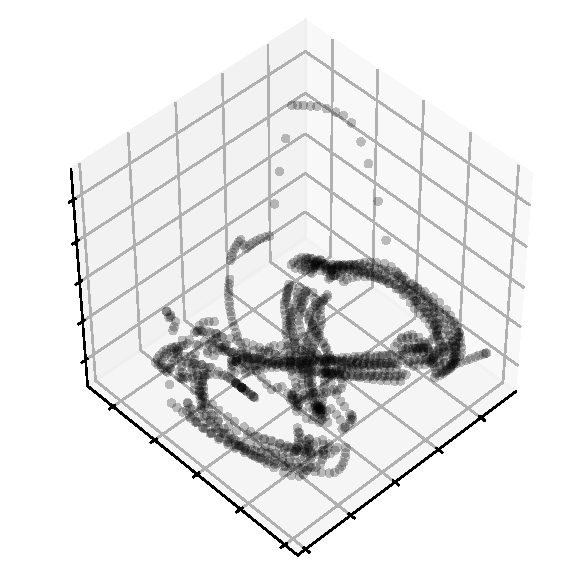
\includegraphics[width=0.75\textwidth]{q3dm1-data-path2.pdf}
\end{center}

Fit a self organizing map of $k=24$ neurons into the given data points $\vec{x}[t]$. This SOM should have the following topological- or \emph{map space} structure
\begin{center}
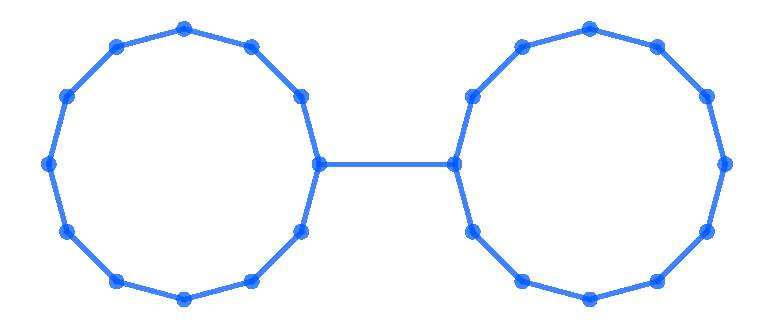
\includegraphics[width=0.6\textwidth]{som-infty-topology.pdf}
\end{center}
\newpage





Plot the data in \texttt{q3dm1-path2.csv} together with the SOM you fitted to it. Plot data points in black and SOM weights and their connections in \textcolor{blue}{blue}.

\textbf{Note:} if your fitted SOM looks ``twisted'', then run the training algorithm again, until you obtain a better fit.
%%%%%
%%%%% enter your answer here, i.e. replace "placeholder.pdf" by the name of the graphics file you created
%%%%%
\begin{center}
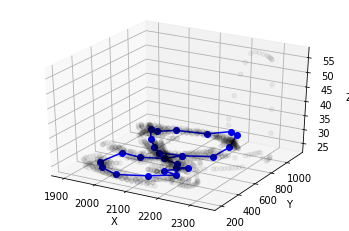
\includegraphics[width=0.7\textwidth]{som24.png}
\end{center}
%%%%%
%%%%%
%%%%%





\vspace{2cm}
Once you have fitted your SOM, determine how well its weights $\vec{w}_1, \ldots, \vec{w}_k$ represent the data. To do this, compute the mean squared error
\begin{equation*}
E = \frac{1}{n} \sum_{t=1}^n \, \min_i \, \dsq{\vec{x}[t]}{\vec{w}_i}
\end{equation*}
Round your result to \emph{two} decimals and enter it here \color{blue}
%%%%%
%%%%% enter your answer after the '=' sign
%%%%%
\begin{equation*}
E = 1671.85
\end{equation*}
%%%%%
%%%%%
%%%%%
%%%%%
\color{black}
\newpage

\color{black}
\subsection*{action primitives from in-game data}

Given the sequence
\begin{equation*}
\vec{x}[1]:\vec{x}[2]:\vec{x}[3]:\vec{x}[3]:\cdots:\vec{x}[n]
\end{equation*}
of subsequent 3D locations contained in file \texttt{q3dm1-path2.csv}, compute a sequence
\begin{equation*}
\vec{v}[1]:\vec{v}[2]:\vec{v}[3]:\vec{x}[3]:\cdots:\vec{v}[n-1]
\end{equation*}
of velocity vectors where 
\begin{equation*}
\vec{v}[t] = \vec{x}[t+1] - \vec{x}[t]
\end{equation*}





\vspace{2cm}
Given your sequence of velocity vectors, compute their average
\begin{equation*}
\mathbb{E} \bigl[ \vec{v} \bigr] = \frac{1}{n-1} \sum_{t=1}^{n-1} \vec{v}[t]
\end{equation*}
Enter your result here. That is, replace the dots in the following expression by the appropriate numbers rounded to \emph{four} decimals. \color{blue}
%%%%%
%%%%% enter your answer here, i.e. replace the \ldots with the numbers you computed
%%%%%
\begin{equation*}
\mathbb{E} \bigl[ \vec{v} \bigr] = \begin{bmatrix} \ldots \\ \ldots \\ \ldots \end{bmatrix}
\end{equation*}
%%%%%
%%%%%
%%%%%
\color{black}





\vspace{2cm}
Run $k$-means clustering on the velocity vectors $\vec{v}[t]$ to estimate representative velocities or \emph{action primitives} $\vec{a}_1, \vec{a}_2, \ldots, \vec{a}_k$. For $k=24$, compute the average
\begin{equation*}
\mathbb{E} \bigl[ \vec{a} \bigr] = \frac{1}{k} \sum_{i=1}^{k} \vec{a}_i
\end{equation*}
Enter your result here. That is, replace the dots in the following expression by the appropriate numbers rounded to \emph{four} decimals. \color{blue}
%%%%%
%%%%% enter your answer here, i.e. replace the \ldots with the numbers you computed
%%%%%
\begin{equation*}
\mathbb{E} \bigl[ \vec{a} \bigr] = \begin{bmatrix} \ldots \\ \ldots \\ \ldots \end{bmatrix}
\end{equation*}
%%%%%
%%%%%
%%%%%
\color{black}

\end{document}
